\chapter{Background Theory - Deep Learning}
\label{chap:Theory-Deep Learning}
\section{Introduction to Machine Learning and Deep Learning}
Machine Learning is a branch of artificial intelligence that focuses on developing algorithms capable of learning from data and improving their performance over time. While traditional rule-based programming has explicit instructions to solve a problem, machine learning algorithms autonomously discover patterns and insights from data without being programmed for each task. The learning process utilizes statistical models and optimization algorithms to iteratively adjust parameters and improve performance. Machine learning encompasses various approaches, including supervised learning, unsupervised learning, and reinforcement learning based on types of data and learning objectives. \\

\textbf{Supervised learning} involves training a model using labeled data, where each input is paired with a corresponding output. During training, the model learns to map input data to output labels by minimizing the difference between its predictions and the true labels. This approach is commonly used for tasks such as classification and regression, where the goal is to learn a mapping from inputs to outputs based on example pairs. \\

\textbf{Unsupervised learning}, in contrast, involves training a model on unlabeled data, where the algorithm aims to find hidden patterns or structures within the data without explicit guidance. Unsupervised learning is often used for tasks like anomaly detection, data exploration, and feature learning, where the data lacks labeled examples or where the underlying structure is unknown. \\

In \textbf{Reinforcement learning}, an agent learns to make decisions by interacting with an environment to maximize cumulative rewards. The agent learns through trial and error, receiving feedback from the environment in the form of rewards or penalties for its actions. By exploring different actions and their consequences, the agent gradually improves its decision-making policy to achieve long-term goals. \\

Deep Learning is a subset of machine learning that has gained significant attention due to its remarkable performance in various tasks, ranging from image and speech recognition to natural language processing and autonomous driving. Deep Learning models utilizes neural networks consisting of multiple layers of interconnected neurons to learn representations of data. These representations, learned through iterative processing of input data, enable the model to extract complex patterns and make predictions or decisions. The key distinction between machine learning and deep learning lies in the depth and complexity of the models. While machine learning approaches may require feature engineering to extract relevant information from raw data, deep learning models learn feature representations directly from the data, making them more adaptable to diverse and high-dimensional datasets. \\
We will exclusively delve into the specifics of supervised learning in this work. Henceforth, when we mention machine learning or deep learning, it refers to supervised learning in this context.
\section{Fundamentals of Neural Networks}
Artificial Neural Networks (ANNs) are computational models inspired by the structure and function of biological neural networks. They consist of interconnected nodes organized into layers, typically including an input layer, one or more hidden layers, and an output layer. ANNs are capable of learning complex patterns from data through iterative processing. \\
A \textbf{perceptron} or an artificial neuron, inspired by biological neurons in the brain, is the fundamental building block of ANNs. It takes multiple input signals $\mathbf{x}= \left(x_1, x_2 ...x_n\right)$, each weighted by a connection weight $w_1,w_2,...w_n$, sums them up, and applies an activation function $\sigma$ to produce an output $\mathbf{y} = \sigma \left(\mathbf{w}^T\mathbf{x} + \mathbf{b} \right)$, where $\mathbf{b}$ is the bias. Perceptrons are arranged in layers to build complex neural network architectures.\\
\begin{figure}[ht]
    \centering
    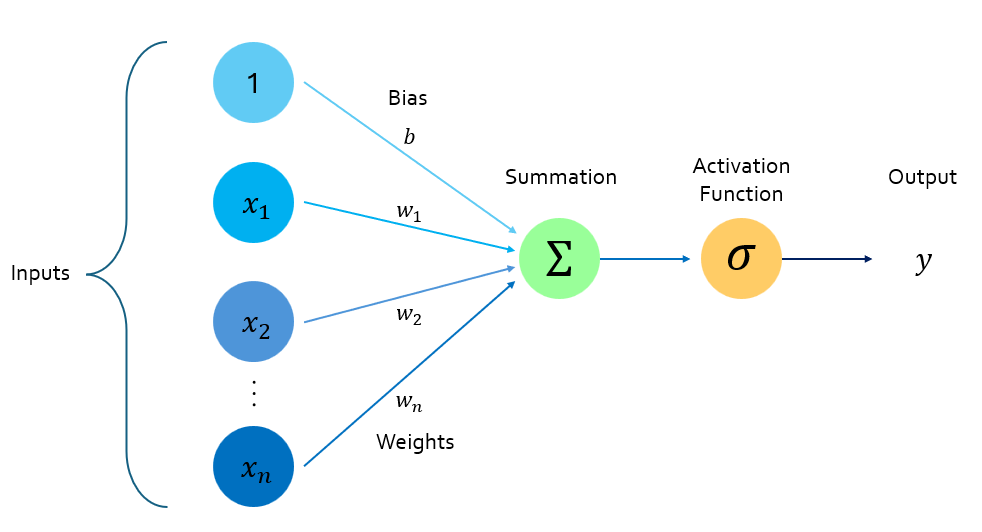
\includegraphics[width=10cm]{images/Theory-DL/ActFn.png}
    \caption{Perceptron}
    \label{fig:Perceptron}
  \end{figure}
\textbf{Activation functions} are usually non-linear functions to introduce non-linearity within the layers of neural networks, allowing them to learn and represent complex relationships in data. Common activation functions include sigmoid, tanh, ReLU (Rectified Linear Unit), and softmax. For example, the sigmoid activation function is defined as $\sigma\left(\mathbf{z}\right)$, where $\mathbf{z} = \mathbf{w}^T\mathbf{x} + \mathbf{b}$ is the weighted sum of inputs and bias term. Activation functions transform the input signal $\mathbf{z}$ into the output signal $\mathbf{y}$, typically in the range between 0 and 1 (for sigmoid) or -1 and 1 (for tanh), enabling the network to capture and model more intricate patterns. Without this nonlinear transformation via the activation function, the network would be confined to solving merely linear problems. Selecting an appropriate activation function is critical and is one of
the hyperparameters in a learning algorithm. Further explanation about hyperparameters is discussed in \ref{section:hyperparameters}.\\
\begin{figure}[ht]
    \centering
    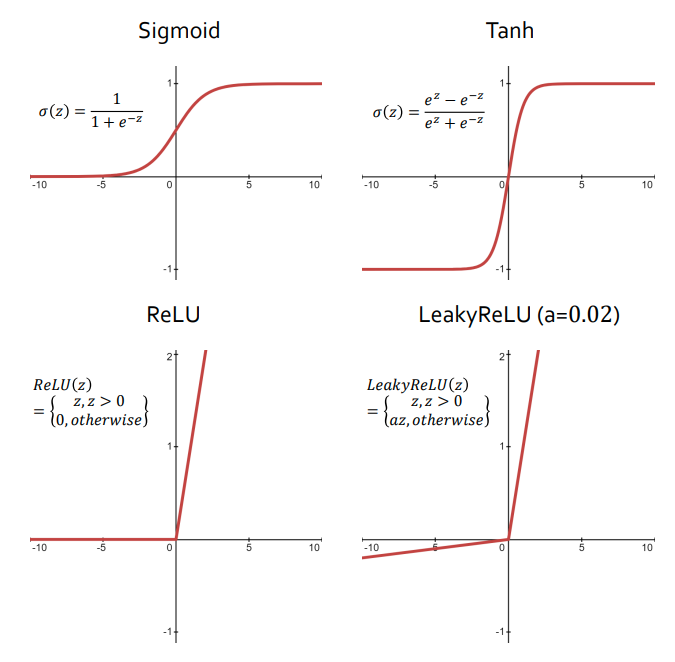
\includegraphics[width=10cm]{images/Theory-DL/ActGraphs.png}
    \caption{Activation functions: (a) Sigmoid, (b) Tanh, (c) ReLU, and (d) Leaky ReLU}
    \label{fig:ActGraphs}
  \end{figure}
\textbf{Weights} in a neural network represent the strength of connections between neurons. They are learned parameters to adjust the influence of input signals on the neuron's output. \textbf{Biases} allow neural networks to model the offset from zero output, influencing the activation of neurons regardless of the input.\\
\textbf{Neural networks (NNs)} consist of interconnected layers of perceptrons that process input data to produce output predictions. NNs can be represented as directed graphs, where nodes correspond to artificial neurons, and edges depict connections between them. These connections typically carry weighted signals from one neuron's output to another neuron's input. Based on the structure of this connection graph, neural networks can be broadly classified into two categories, feed-forward neural networks and recurrent neural networks.\\
In \textbf{feed-forward neural networks}, information flows only in one direction, from the input layer through one or more hidden layers to the output layer. Each layer processes the input data independently, and the output of one layer serves as the input to the next layer. The connections between neurons do not form directed cycles, ensuring that the network architecture is acyclic. Multi Layer Perceptrons (MLPs) are the simplest feed-forward neural networks and their architecture is described in the Figure \ref{fig:MLP}. \\
\begin{figure}[ht]
    \centering
    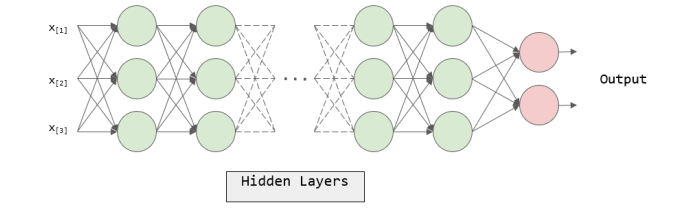
\includegraphics[width=10cm]{images/Theory-DL/MLP.png}
    \caption{Architecture of a Multi Layer Perceptron}
    \label{fig:MLP}
  \end{figure}
\textbf{Recurrent neural networks}, on the other hand, are designed to handle sequential data by allowing connections between neurons to form directed cycles. This architecture enables them to exhibit temporal dynamics and capture dependencies across time steps in sequential data. The feedback loops in RNNs allow the network to maintain a memory of past inputs, making them suitable for tasks involving sequential data, such as natural language processing, time series prediction, and speech recognition.
\section{Optimization}
Optimization involves adjusting the parameters of the neural network, such as weights and biases, to minimize a predefined objective function, typically referred to as the loss function. The optimization process iteratively updates the parameters based on the gradients of the loss function with respect to the network's parameters, aiming to converge to a set of optimal parameters that yield the best performance on the given task.
\subsection{Loss Function}
The loss function, also known as the objective function or cost function, quantifies the difference between the model's predictions and the actual target values. It represents the measure of how well the model is performing on the training data. Common loss functions include mean squared error (MSE) for regression tasks and categorical cross-entropy for classification tasks. Mathematically, the loss function $\mathcal{L}(\theta)$ is defined as: 
\begin{equation}
    \mathcal{L}(\theta)=\frac{1}{N} \sum_{i=1}^N L\left(y_i, \hat{y}_i ; \theta\right)
    \end{equation}
Here, $\theta$ represents the parameters of the neural network being optimized, such as weights and biases, $y_i$ is the ground truth and $\hat{y}_i $ is the model prediction. The loss function $\mathcal{L}(\theta)$ depends on these parameters, and it is computed as the average of the individual loss $L\left(y_i, \hat{y}_i ; \theta\right)$ over all training examples.
\subsection{Backpropagation}
Backpropagation is a fundamental algorithm used to compute the gradients of the loss function with respect to the parameters (weights and biases) of the neural network. It involves propagating the error backward from the output layer to the input layer, updating the parameters along the way to minimize the loss. The gradients are computed using the chain rule of calculus, enabling efficient optimization of the network's parameters. Mathematically, the gradients of the loss function $\nabla_\theta \mathcal{L}(\theta)$ with respect to the parameters $\theta$ are computed recursively using the chain rule.
\begin{equation}
    \nabla_\theta \mathcal{L}(\theta)=\frac{1}{N} \sum_{i=1}^N \nabla_\theta L\left(y_i, \hat{y}_i ; \theta\right)
    \end{equation}
Here, $\nabla_\theta L\left(y_i, \hat{y}_i ; \theta\right)$ represents the gradient of the loss function with respect to the parameters for each training example.
\begin{figure}[ht]
    \centering
    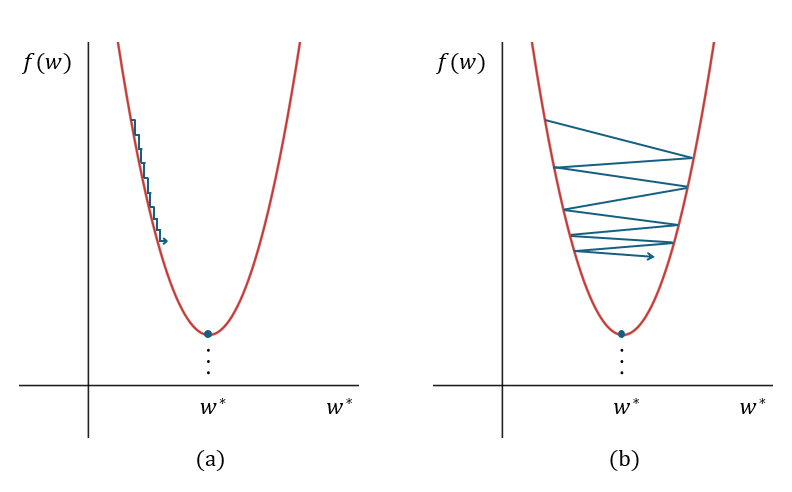
\includegraphics[width=10cm]{images/Theory-DL/LR.png}
    \caption{Effect of Learning Rates}
    \label{fig:LR}
    \end{figure}
\subsection{Learning Rate}
The learning rate is a hyperparameter that controls the size of the parameter updates, that is the step size in the direction of the gradients computed by backpropagation. A higher learning rate may lead to faster convergence but risks overshooting the optimal solution, while a lower learning rate may result in slower convergence but more stable training, as seen in Figure \ref{fig:LR}. The parameter update rule with learning rate $\eta$ is given by:
\begin{equation}
    \theta_{t+1}=\theta_t-\eta \nabla_\theta \mathcal{L}(\theta)
    \end{equation}
Here, $\theta_{t+1}$ and $\theta_t$ represent the parameters at time step $t$ and $t+1$ respectively, and $\mathcal{L}(\theta)$ is the gradient of the loss function with respect to the parameters. Adjusting the learning rate appropriately is essential for achieving optimal performance and preventing issues such as divergence or slow convergence during training. Learning rate decay is often used to gradually reduce the learning rate during training. There are several types of learning rate schedulers commonly used in deep learning: \\
\textbf{Step Decay} reduces the learning rate by a factor (typically constant) after a fixed number of epochs or iterations as $\eta_{new} = \eta_{old} \times \mathbf{df}$, where, $\eta_{new}$ and $\eta_{new}$ are the current and previous learning rates respectively and $\mathbf{df}$ is a hyperparameter determining the rate of decay. \\
\textbf{Exponential decay} reduces the learning rate exponentially over time, updated as $\eta_{new} = \eta_{old} \times \mathbf{df}^{\frac{\text{epoch}}{\text{steps}}}$, where $epoch$ is the current epoch, and $steps$ is a parameter specifying how often the decay should occur. \\
\textbf{Cosine Annealing} gradually reduces the learning rate according to a cosine function. \\
\textbf{ReduceLROnPlateau} reduces the learning rate by a factor after a certain number of epochs when a metric (e.g., validation loss) has stopped improving.
\subsection{Optimizer}
The optimizer is responsible for updating the parameters of the neural network based on the gradients computed during backpropagation. It determines the direction and magnitude of parameter updates to minimize the loss function efficiently. These optimizers adjust the learning rates of individual parameters based on their past gradients and update rules, allowing for faster convergence and improved performance. Popular optimizers include stochastic gradient descent (SGD), Adam, RMSprop, and AdaGrad. \\
\textbf{Stochastic Gradient Descent (SGD)} updates the model parameters in the opposite direction of the gradient of the loss function with respect to the parameters. SGD performs parameter updates using a fixed learning rate, which can lead to oscillations or slow convergence, especially in the presence of sparse or noisy gradients.\\
\textbf{RMSprop (Root Mean Square Propagation)} adapts the learning rate for each parameter based on the magnitudes of recent gradients. It maintains a moving average of squared gradients for each parameter and divides the learning rate by the square root of this average to scale the parameter updates. RMSprop helps mitigate the issues of oscillations and slow convergence associated with fixed learning rates in SGD.\\
\textbf{AdaGrad (Adaptive Gradient Algorithm)} adapts the learning rate for each parameter based on the historical gradients accumulated during training. It scales the learning rate inversely proportional to the square root of the sum of squared gradients, effectively giving larger updates to parameters with smaller gradients and vice versa. AdaGrad is particularly useful for sparse data or problems with varying feature scales, as it automatically adjusts the learning rates for different parameters.\\
\textbf{Adam (Adaptive Moment Estimation)} combines the benefits of both RMSprop and momentum optimization techniques. It maintains exponentially decaying moving averages of past gradients and past squared gradients for each parameter. Adam also incorporates bias correction terms to compensate for the initial bias towards zero at the beginning of training. The parameter update rule for Adam is given by
\begin{equation}
    \theta_{t+1}=\theta_t-\frac{\eta}{\sqrt{\hat{v}_t}+\epsilon} \cdot \hat{m}_t
    \end{equation}
where, $\hat{m}_t$is the bias-corrected estimate of the first moment (mean) of the gradients, $\hat{v}_t$ is the bias-corrected estimate of the second moment (uncentered variance) of the gradients, and $\epsilon$ is a small constant to prevent division by zero. Adam's adaptive learning rate and momentum updates make it well-suited for a wide range of deep learning tasks, providing fast convergence and robust performance across different architectures and datasets.
\section{Training of Neural Networks}
\subsection{Data Partitioning}Data partitioning is a crucial step in deep learning where the available dataset is divided into separate subsets for training, validation, and testing. Typically, the data is partitioned into training data used to train the model, validation data used to tune hyperparameters and monitor performance, and testing data used to evaluate the final model's generalization performance. The partitioning process ensures that the model's performance is assessed accurately on unseen data and helps prevent overfitting by providing independent datasets for training and evaluation. 
\subsection{Feature Scaling}Feature scaling or normalization is a preprocessing step aimed at bringing all input features to a similar scale. Features with large magnitudes can lead to large gradients during training, which may cause unstable behavior and make it challenging for the optimization algorithm to find the optimal solution. Feature scaling mitigates this issue by reducing the range of feature values, thus preventing gradient instability and ensuring more reliable optimization. Normalizing features to a standard scale also makes the model less sensitive to variations in the input data distribution, leading to better generalization performance on new, unseen samples. Additionally, scaling features to a common range ensures that each feature contributes equally to the learning process, preventing bias towards certain features. Common methods of feature scaling include
\begin{enumerate}
\item Min-Max Normalization: $x^{\prime}=\frac{x-x_{\min }}{x_{\max }-x_{\min }}$
\item Z-Score Standardization: $x^{\prime}=\frac{x-\tilde{x}}{\sigma}$
\item Unit Length Scaling: $\mathrm{x}^{\prime}=\frac{\mathrm{x}}{\|\mathrm{x}\|}$
\end{enumerate}
\subsection{Weights Initialization}
Weight initialization is a crucial aspect of training neural networks, as it sets the starting values for the model's parameters (weights) before training begins. While the neural network does learn optimal values for the weights during training, the choice of initial weights significantly influences the convergence speed and performance of the network as the loss landscape of deep neural networks is high-dimensional and non-convex, with multiple local minima. The aim is to apply a good weight initialization that can guide the optimization algorithm towards more favorable regions of the loss surface, facilitating faster convergence to better solutions. There are different cases to consider for weight initialization: 
\begin{enumerate}
\item Initializing all weights to 0 or a constant leads to symmetrical gradients and symmetric weight updates across all neurons in the network during backpropagation. This results in the neurons learning identical features, causing the network to lose its representational capacity and fail to learn complex patterns. This results in poor convergence and suboptimal performance.
\item Initializing weights to large values can lead to exploding gradients during training. When weights are large, activations and gradients become large as well, causing unstable updates and divergence in optimization. Additionally, large weights can saturate activation functions, pushing them into regions of zero gradients (e.g., in sigmoid or tanh activations), hindering learning and resulting in slow convergence.
\item Initializing weights to small values helps prevent exploding gradients, as activations and gradients remain within a manageable range during training. However, if weights are initialized too small, activations may also become small, leading to vanishing gradients. This can impede learning, especially in deep networks with many layers, where gradients diminish exponentially as they propagate backward. 
\item Initializing weights to random values drawn from a suitable distribution, such as a normal distribution with zero mean and small variance, is a common practice. Random initialization breaks symmetry and helps prevent both vanishing and exploding gradients. It encourages each neuron to learn different features from the input data, promoting diverse representations and effective learning.
\end{enumerate}
In summary, weight initialization is crucial for initializing neural networks effectively. Random initialization is preferred, as it breaks symmetry, prevents vanishing/exploding gradients, and enables efficient training by promoting diverse feature learning. Techniques like Xavier and Kaiming initialization further refine this process by adapting to the specific characteristics of activation functions and network architectures.
\subsubsection{1. Xavier Initialization (Glorot Initialization):}
\begin{itemize}
  \item This technique initializes weights from a distribution with zero mean, typically a normal or uniform distribution, to ensure stable training. The variance of the distribution is adjusted based on the number of input and output neurons, known as fan-in and fan-out, respectively.
  \[ \text{Var}(W) = \frac{2}{\text{fan}_{\text{in}} + \text{fan}_{\text{out}}} \]
  \item Xavier initialization is commonly used in shallow networks with symmetric activation functions, ensuring balanced weight initialization and stable training dynamics.
  \item \textbf{Application:} Xavier initialization is suitable for fully connected layers and shallow neural networks with symmetric activation functions like tanh or sigmoid.
  \item \textbf{Limitations:} This method is not optimal for non-symmetric activations like ReLU.
\end{itemize}
\subsubsection{2. Kaiming Initialization (He Initialization):}
\begin{itemize}
  \item Kaiming initialization is designed for networks using non-linear activations like ReLU as seen in modern deep learning architectures.
  \item It initializes weights from a normal distribution with zero mean, adjusting the variance based on fan-in.
  \[ \text{Var}(W) = \frac{2}{\text{fan}_{\text{in}}} \]
  \item Kaiming initialization helps mitigate the issue of vanishing gradients associated with ReLU activations, ensuring stable training and faster convergence.
  \item \textbf{Application:} Kaiming initialization is widely used in deep neural networks with non-linear activations like ReLU.
  \item \textbf{Advantages:} It leads to improved convergence and model performance that use ReLU activations or its variants.
\end{itemize}
\subsection{Regularization}
Regularization broadly refers to techniques used to prevent overfitting by imposing additional constraints on the model's parameters, i.e; by adding penalties to the loss function, thus discouraging complex models. Regularization penalizes large weights in the model, thereby promoting simpler models that generalize better to unseen data. Two common forms of regularization are L1 regularization (Lasso) and L2 regularization (Ridge). \\
L1 regularization encourages sparsity in the weight vector, effectively performing feature selection by setting irrelevant weights to zero, making the model simpler and more interpretable. 
\[ \operatorname{Loss}_{\mathrm{L} 1}=\operatorname{Loss}_{\text {original }}+\lambda \sum_{i=1}^n\left|w_i\right| \]
L2 regularization encourages the distribution of weights to be spread out more evenly, preventing individual weights from becoming too large, improving the generalization performance of the model.
\[ \operatorname{Loss}_{\mathrm{L} 2}=\operatorname{Loss}_{\text {original }}+\lambda \sum_{i=1}^n w^2_i \]
The regularization strength $\lambda$ determines the degree of penalty imposed on large weights. A smaller $\lambda$ value results in weaker regularization, allowing the model to fit the training data more closely but increasing the risk of overfitting. Conversely, a larger $\lambda$ value increases the regularization effect, leading to smaller weights and a simpler model that generalizes better to unseen data but may underfit the training data if set too high.
\subsection{Dropout}
Dropout is a regularization technique used in neural networks during training, where a random fraction of neurons is temporarily dropped out or ignored during forward and backward propagation. This prevents neurons from co-adapting and overfitting to the training data, promoting robustness and generalization.
\subsection{Batch Training and Batch Normalization}
Batch training is a technique in deep learning in which the model updates its parameters based on a subset (or batch) of the training data, rather than the entire dataset. The training data is divided into batches of fixed size, and the model computes the gradients of the loss function with respect to the parameters for each batch using backpropagation. 
\subsubsection{Advantages}
\begin{itemize}
    \item The major advantage of batch training is that it computes the gradient updates based on an average over the samples in each batch, which reduces the variance in the gradient estimates compared to processing the entire dataset at once. This averaging effect stabilizes the gradients and prevents large fluctuations during training. 
    \item Batch training allows for efficient memory utilization by processing only a subset of the dataset at a time. This is especially advantageous for large-scale datasets that cannot fit entirely into memory. By processing data in batches, the memory requirements are significantly reduced, enabling training on datasets that would otherwise be impractical to handle. 
\end{itemize}
Selecting an appropriate batch size is crucial, as too small a batch size can introduce high variance in parameter updates, while too large a batch size may result in slower convergence and potential overfitting. Smaller batch sizes lead to more frequent updates and noisier gradients, which can aid in escaping local minima but may slow convergence. They introduce randomness into training, acting as a form of regularization to prevent overfitting. Conversely, larger batch sizes provide more precise gradient estimates, leading to more stable optimization and faster convergence, but require more computational resources and memory. Finding the optimal batch size involves balancing the trade-off between computational efficiency and the quality of gradient estimates. \\                     
Another important term in this context is an epoch, which refers to a single pass through the entire training dataset. During one epoch, the entire training dataset is divided into batches, and each batch is processed sequentially through the neural network. Once all batches have been processed, completing one full iteration over the entire dataset, one epoch is considered complete. Typically, training iterates over the entire dataset for multiple times or epochs until the model converges or until a predefined stopping criterion is met. Batch training involves updating model parameters based on the gradients computed over batches, while epoch defines the number of times the training algorithm iterates over the entire dataset. \\
% Batch normalization (BatchNorm) is another technique used in deep learning to stabilize and accelerate training by normalizing the activations of each layer within a mini-batch. 
Batch normalization (BatchNorm) is another technique to improve the stability and performance of neural networks by normalizing the activations of each layer. Batch normalization operates on mini-batches of data within each layer with the main idea of normalizing the input of each layer to have a mean of zero and a standard deviation of one, thereby reducing internal covariate shift. This is achieved by computing the mean and standard deviation of the activations across the batch and then scaling and shifting the activations using learned parameters. BatchNorm improves gradient flow, enables higher learning rates, and acts as a regularizer, leading to faster convergence and improved generalization performance. Mathematically, for a mini-batch $B$ of size $m$, with input $x^{(1)}, x^{(2)}, \ldots, x^{(m)}$, the batch normalization transformation for a layer is as follows:
\begin{equation}
\begin{aligned}
& \mu_B=\frac{1}{m} \sum_{i=1}^m x^{(i)} \\
& \sigma_B^2=\frac{1}{m} \sum_{i=1}^m\left(x^{(i)}-\mu_B\right)^2 \\
& \hat{x}^{(i)}=\frac{x^{(i)}-\mu_B}{\sqrt{\sigma_B^2+\epsilon}} \\
& y^{(i)}=\gamma \hat{x}^{(i)}+\beta
\end{aligned}
\end{equation}
where $\mu_B$ and $\sigma_B^2$ are the mean and variance of the mini-batch $B, \epsilon$ is a small constant added to avoid division by zero, $\hat{x}^{(i)}$ is the normalized input, $\gamma$ and $\beta$ are learnable parameters (scale and shift), and $y^{(i)}$ is the output of the batch normalization layer.
\subsection{Underfitting and Overfitting}
Overfitting and underfitting are two common phenomena that affect the performance and generalization ability of machine learning models. Overfitting occurs when a model learns to perform well on the training data but fails to generalize to unseen data. This happens when the model captures noise or random fluctuations in the training data as if they were genuine patterns. As a result, the model becomes overly complex and specific to the training set, leading to poor performance on new, unseen data. Signs of overfitting include high training accuracy but low validation or test accuracy, and the model may exhibit excessively complex decision boundaries or memorize training examples. \\
Underfitting, on the other hand, occurs when a model is too simple to capture the underlying structure of the data. In this case, the model fails to learn the patterns present in the training data and performs poorly both on the training and unseen data. Underfitting often occurs when the model is too shallow or lacks the necessary complexity to represent the data adequately. It can also occur when the model is trained for too few epochs or with insufficient training data. Signs of underfitting include low training and validation accuracy, as well as a high bias or inability to capture the complexity of the data.\\
Addressing these issues often involves finding the right balance between model complexity and the amount of available training data. Techniques such as regularization, dropout, early stopping, and hyperparameter tuning can help prevent overfitting by reducing the model's capacity or complexity. Conversely, increasing the model's capacity, adding more data, or improving feature engineering can help alleviate underfitting by allowing the model to capture more complex relationships in the data.
\subsection{Hyperparameters}\label{section:hyperparameters}
Hyperparameters in machine learning and deep learning are parameters that are set prior to the training process and are not learned from the data. They control various aspects of the learning process, such as the architecture of the model, the optimization algorithm used, and the training procedure itself. Some important hyperparameters are number of neurons per layer, number of layers, activation function, batch size, number of epochs, optimizer, loss function, weight initialization, dropout rate, and regularization strength. \\
Hyperparameter tuning, also known as hyperparameter optimization, is the process of selecting the optimal values for these hyperparameters to maximize the performance of the model on unseen data. It involves systematically searching through a predefined space of hyperparameters and evaluating the model's performance using a validation set or cross-validation. The goal is to find the hyperparameters that result in the best generalization performance, balancing between underfitting and overfitting.
\subsubsection{K-Fold Cross Validation}
In K-fold cross-validation, the dataset is divided into K subsets, or folds, of approximately equal size. The model is trained K times, each time using K-1 folds for training and the remaining fold for validation. This process is repeated K times, with each fold used exactly once as the validation set. In the context of hyperparameter tuning, K-fold cross-validation helps evaluate the performance of different hyperparameter configurations more accurately. Instead of relying on a single validation set, which may be sensitive to the particular random split of the data, K-fold cross-validation averages the performance over multiple folds, providing a more stable estimate of the model's performance.
\section{Model Evaluation Metrics}
Model evaluation metrics are essential for assessing the performance of deep learning models and understanding how well they generalize to unseen data. The loss function serves as a crucial metric for evaluating model performance, in addition to optimizing model parameters during training. In regression tasks, where the goal is to predict continuous values, common loss functions include Mean Absolute Error (MAE), Mean Squared Error (MSE), and Root Mean Squared Error (RMSE).
\begin{itemize}
\item \textbf{Mean Absolute Error (MAE):} MAE measures the average absolute difference between the predicted values and the actual values:\[ \text{MAE} = \frac{1}{n} \sum_{i=1}^{n} |y_i - \hat{y}_i| \] Here, $y_i$ are the ground truth values, $\hat{y}_i$ are the predicted values, and $n$ is the number of samples. MAE is robust to outliers butdoes not penalize large errors as heavily as MSE or RMSE.
% \textbf{Mean Relative Error (MRE)}
\item \textbf{Mean Squared Error (MSE):} MSE measures the average squared difference between the predicted values and the actual values:\[ \text{MSE} = \frac{1}{n} \sum_{i=1}^{n} (y_i - \hat{y}_i)^2 \] MSE penalizes larger errors more heavily than MAE since errors are squared. This makes it more sensitive to outliers. MSE is commonly used in optimization algorithms due to its differentiability properties.
\item \textbf{Root Mean Squared Error (RMSE):} RMSE is the square root of the average squared difference between the predicted values and the actual values: \[ \text{RMSE} = \sqrt{\frac{1}{n} \sum_{i=1}^{n} (y_i - \hat{y}_i)^2} \]RMSE provides a measure of the average magnitude of error, similar to MSE, but in the same units as the target variable. RMSE is sensitive to outliers, similar to MSE, but is more interpretable as it is in the same units as the target variable.
\end{itemize}
\section{Convolutional Neural Networks (CNNs)}
CNNs are specialized neural networks designed to process grid-like data, such as images. They utilize convolutional layers to automatically and adaptively learn spatial hierarchies of features from input data, making them highly effective for tasks like image classification, object detection, and image segmentation.
\begin{figure}[ht]
    \centering
    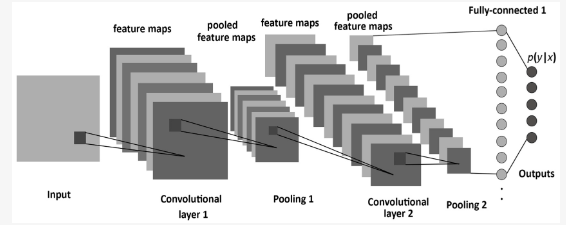
\includegraphics[width=10cm]{images/Theory-DL/CNN.png}
    \caption{Convolutional Neurl Network}
    \label{fig:CNN}
  \end{figure}
\subsection{Convolutional Layer}
The convolutional layer in a CNN consists of a set of learnable filters (kernels) that slide over the input data, performing element-wise multiplication and summing to produce feature maps. The layer preserves the spatial relationship between pixels and learns local patterns like edges, textures, and shapes. 
\begin{figure}[ht]
    \centering
    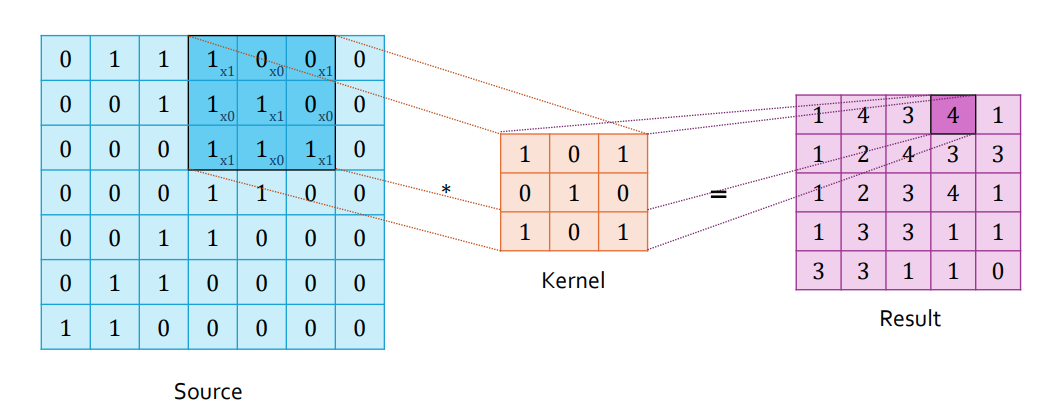
\includegraphics[width=10cm]{images/Theory-DL/Conv1.png}
    \caption{Convolutional Layer}
    \label{fig:Conv1}
  \end{figure}
\begin{figure}[ht]
    \centering
    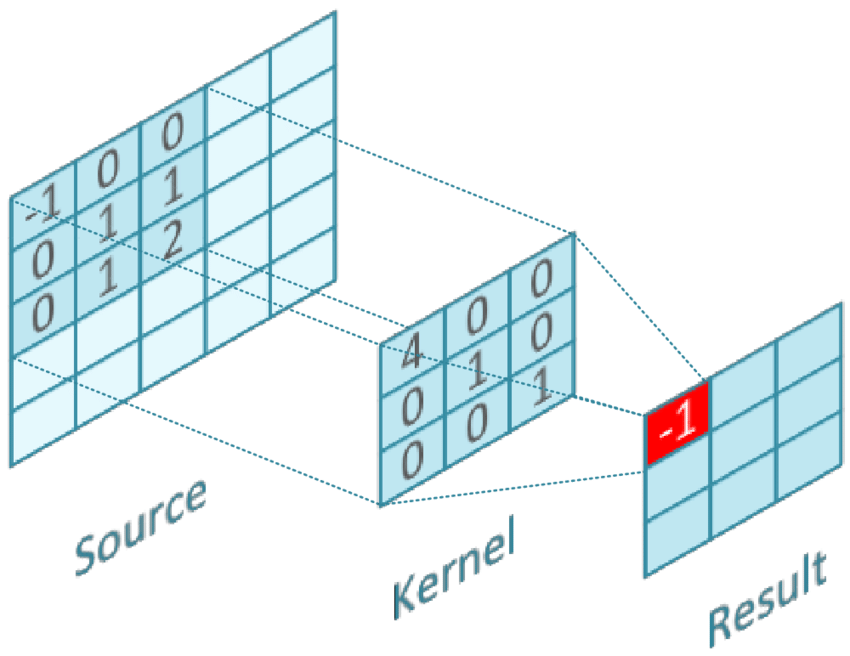
\includegraphics[width=6cm]{images/Theory-DL/Conv2.png}
    \caption{Convolutional Layer}
    \label{fig:Conv2}
\end{figure}
\subsection{Pooling and Unpooling} Pooling and unpooling operators play vital roles in CNNs by facilitating effective down-sampling and up-sampling operations, respectively, enabling hierarchical feature extraction while preserving spatial information. Pooling is a down-sampling operation commonly used in CNNs to reduce the spatial dimensions of feature maps. Max pooling and average pooling are popular pooling techniques, selecting the maximum or average value within each pooling region, respectively. Conversely, unpooling layers, often used in decoding or upsampling, aim to reconstruct the original input resolution from the lower-dimensional representations generated by pooling. These layers typically store the indices of the maximum values during pooling and use them for upsampling. Nearest neighbor interpolation is a simpler upsampling method where each pixel in the input is replicated multiple times to form the output.
\begin{figure}[ht]
    \centering
    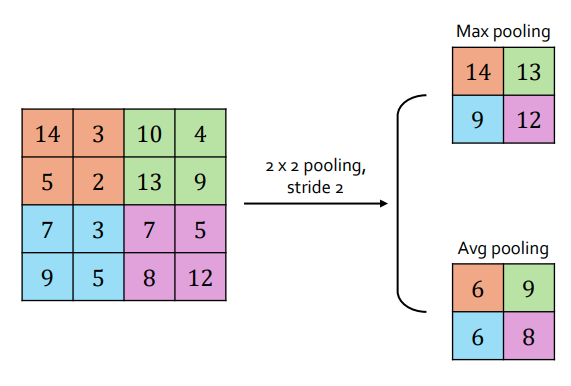
\includegraphics[width=6cm]{images/Theory-DL/Pool.png}
    \caption{Pooling}
    \label{fig:Pool}
\end{figure}\begin{figure}[ht]
    \centering
    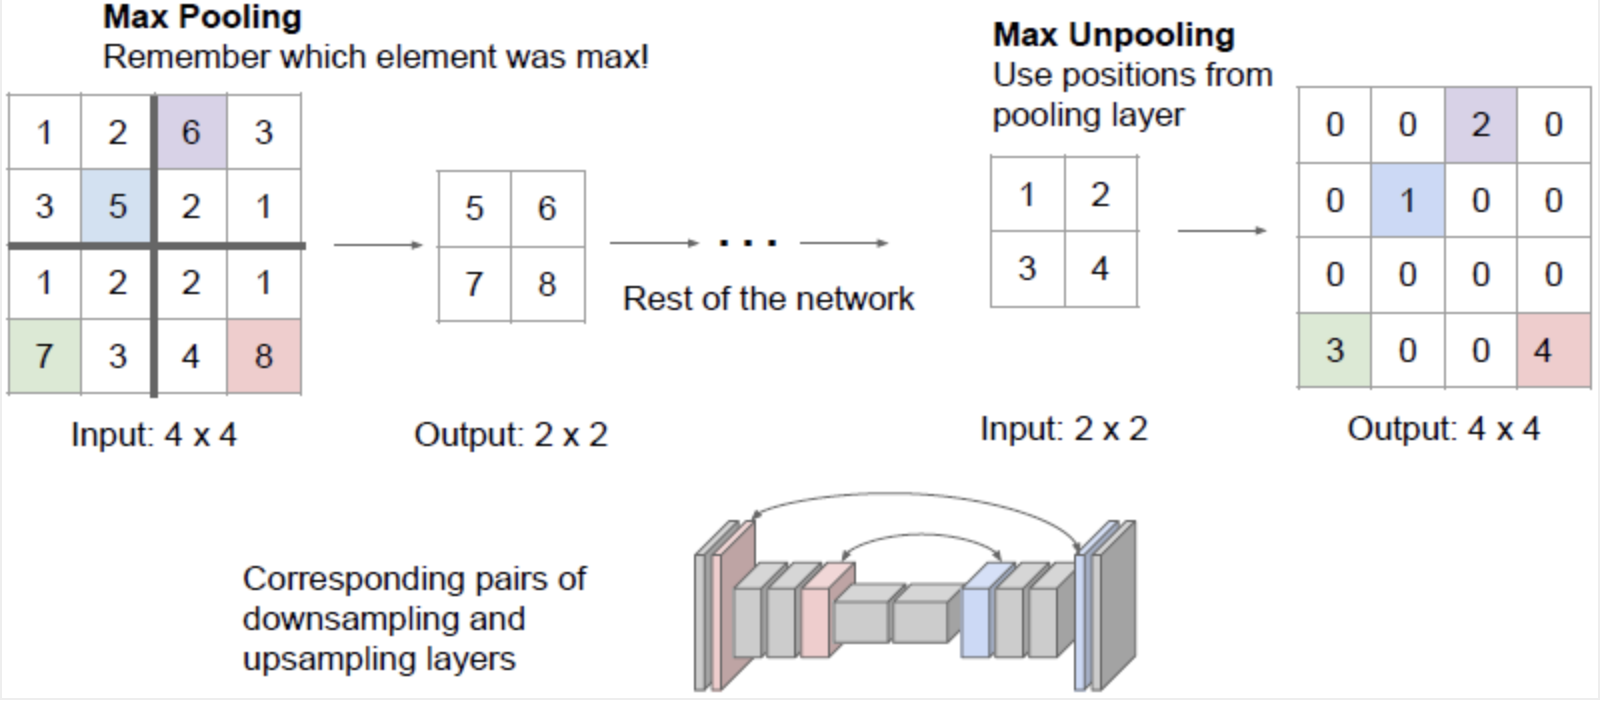
\includegraphics[width=12cm]{images/Theory-DL/MaxUnPool.png}
    \caption{Unpooling}
    \label{fig:Unpool}
\end{figure}    
\begin{figure}[ht]
        \centering
        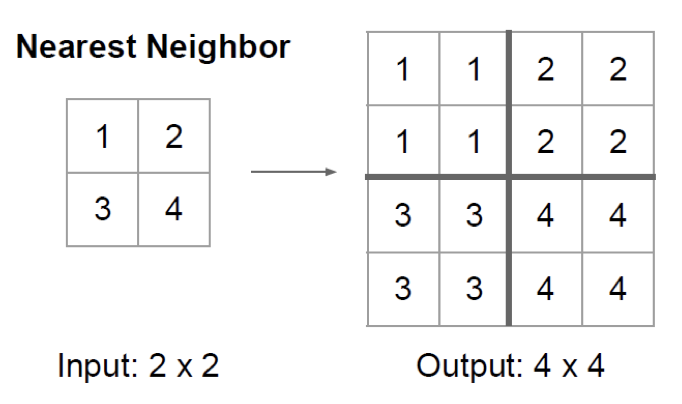
\includegraphics[width=6cm]{images/Theory-DL/NNUnpool.png}
        \caption{Unpooling}
        \label{fig:Unpool2}
    \end{figure}
\subsection{The U-Net Architecture}
The U-Net architecture is a convolutional neural network (CNN) widely used for biomedical image segmentation tasks. It consists of a U-shaped network structure with a contracting path followed by an expanding path, which enables precise segmentation of structures in medical images, such as cells, organs, or tumors. Some important components of the U-Net architecture are discussed below. 
\begin{figure}[ht]
    \centering
    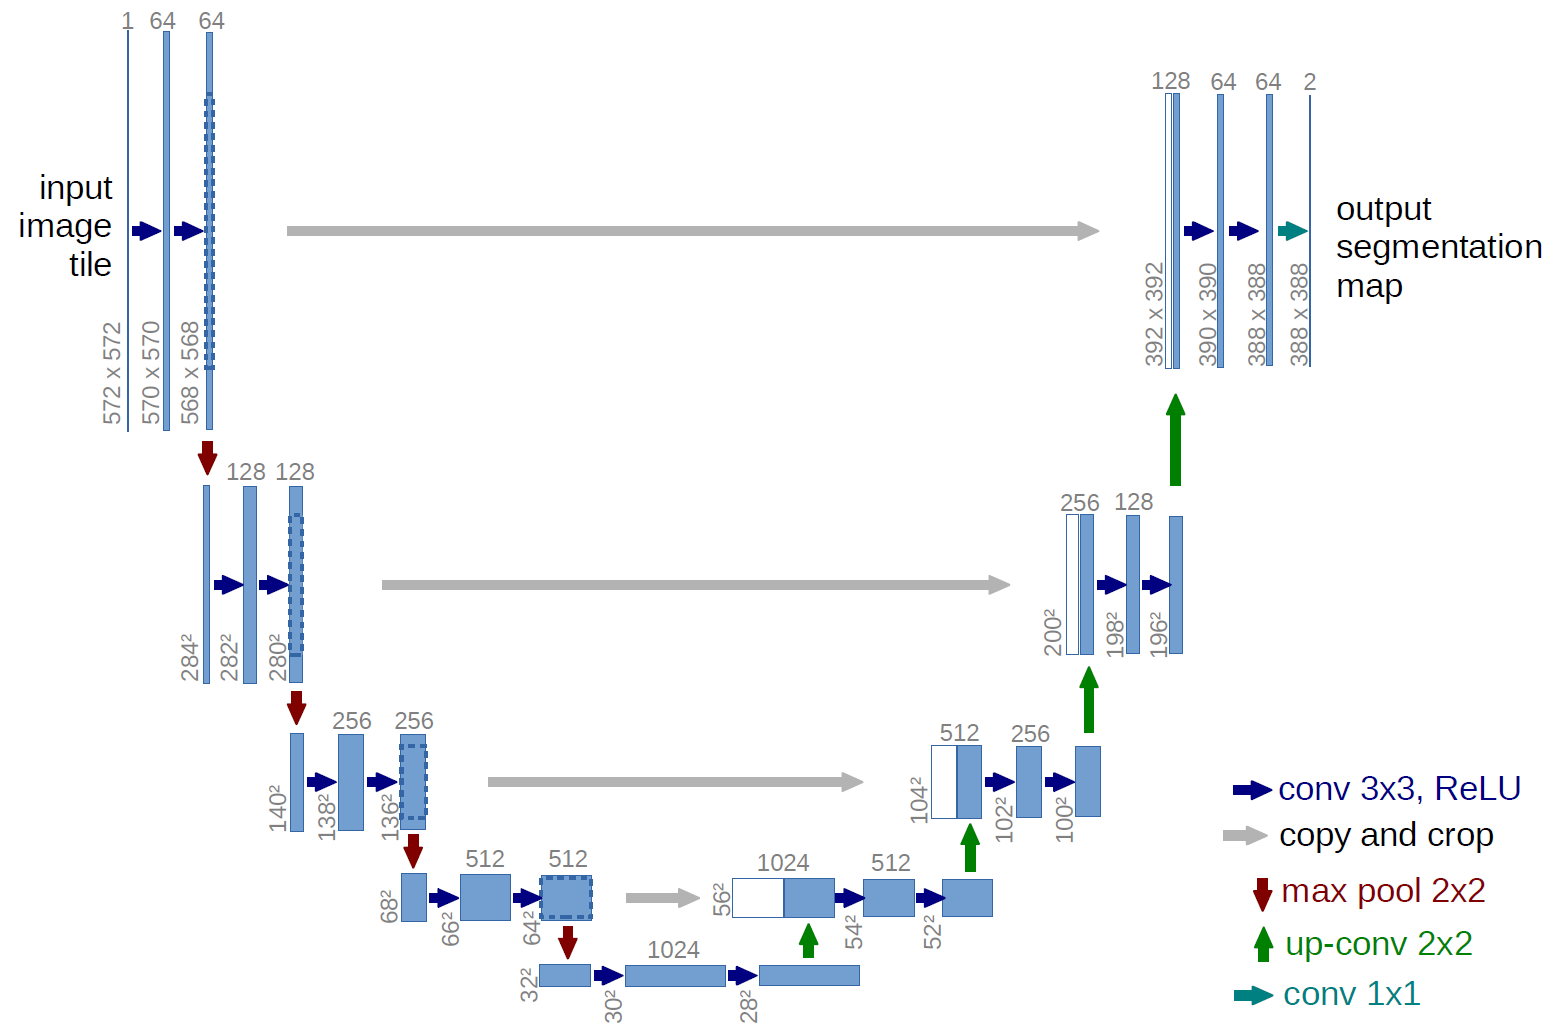
\includegraphics[width=10cm]{images/Theory-DL/UNet.png}
    \caption{U-Net Architecture}
    \label{fig:UNet}
\end{figure}
\begin{enumerate}
  \item \textbf{Contracting Path (Encoder):}
    \begin{itemize}
      \item The contracting path consists of a series of down-convolutional and max-pooling layers that gradually reduce the spatial dimensions of the input image while increasing the number of feature channels.
      \item This path serves as an encoder, extracting high-level features from the input image while preserving spatial context.
    \end{itemize}
  \item \textbf{Expanding Path (Decoder):}
    \begin{itemize}
      \item The expanding path consists of up-convolutional (transposed convolution) and concatenation layers that gradually increase the spatial dimensions of the feature maps while reducing the number of feature channels.
      \item This path serves as a decoder, generating segmentation masks by upsampling the low-resolution feature maps obtained from the contracting path and combining them with high-resolution feature maps from the skip connections.
    \end{itemize}
  \item \textbf{Skip Connections:}
    \begin{itemize}
      \item Skip connections, also known as shortcut connections or residual connections, are direct connections between layers at the same hierarchical level in the network.
      \item In the U-Net architecture, skip connections connect the contracting path (encoder) to the corresponding layers in the expanding path (decoder).
      \item These connections enable the network to retain fine-grained spatial information from the encoder while recovering spatial details lost during downsampling.
      \item By directly linking the encoder and decoder layers, skip connections facilitate the flow of information across different scales, improving the model's ability to capture both local and global context.
    \end{itemize}
\end{enumerate}
\begin{figure}[ht]
    \centering
    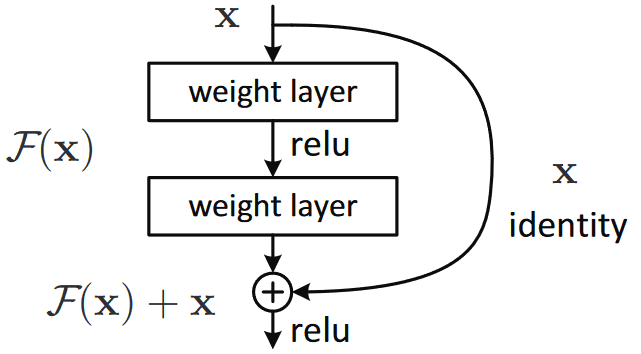
\includegraphics[width=8cm]{images/Theory-DL/Skip.png}
    \caption{Skip Connection}
    \label{fig:Skip}
\end{figure}
A notable observation pertinent to our current endeavor is the striking resemblance between the U-Net architecture and the V-cycle multi-grid method. Both employ a hierarchical structure wherein information is exchanged across varying resolutions.
\section{Graph Neural Networkds (GNNs)}
The development of GNNs can be traced back to the early 2000s, with seminal work by researchers such as Thomas G. Dietterich and Alex J. Smola on graph-based learning algorithms. However, it was not until the mid-2010s that GNNs gained prominence, largely due to the work of researchers like Yoshua Bengio, Jure Leskovec, and Thomas Kipf. In 2016, Kipf and Welling introduced the Graph Convolutional Network (GCN), a foundational architecture that laid the groundwork for modern GNNs. Since then, numerous advancements and variants of GNNs have been proposed, propelling their widespread adoption across various fields. In contrast to CNNs which are well-suited for grid-like structured data such as images, GNNs are tailored for data represented as graphs, which are characterized by non-Euclidean and irregular structures, where entities (nodes) and their relationships (edges) vary in connectivity and structure. GNNs offer several advantages over CNNs, particularly in handling unstructured data. One key limitation of CNNs is their inability to directly operate on irregular data formats, such as social networks, recommender systems, molecular structures, or citation networks. GNNs excel in processing unstructured data by leveraging the inherent graph structure by dynamically aggregating information from neighboring nodes based on their connectivity patterns. CNNs rely on convolutions and pooling operations to extract hierarchical features from grid-like data, whereas GNNs employ message-passing algorithms to aggregate information from neighboring nodes in a graph. This fundamental difference enables GNNs to capture relational information and semantic dependencies inherent in graph-structured data more effectively than CNNs. Some important aspects of GNNs are message passing, graph convolutions and graph pooling which will be discussed in the upcoming section. Graphs are set up using nodes, edges, adjacency matrices, node attributes, and edge attributes. 
\begin{enumerate}
  \item \textbf{Nodes (\(V\))}: Nodes represent entities in a graph, such as users in a social network, atoms in a molecule, or words in a document. Formally, a graph can be denoted as \( G = (V, E) \), where \( V \) is the set of nodes.
  
  \item \textbf{Edges (\(E\))}: Edges define relationships or connections between nodes in a graph. Each edge \( e_{ij} \) connects node \( v_i \) to node \( v_j \), where \( v_i, v_j \in V \). The edge set \( E \) can be represented as a collection of tuples \( (v_i, v_j) \) indicating the connections between nodes.
  
  \item \textbf{Adjacency Matrix (\(A\))}: An adjacency matrix is a binary $n \times n$ matrix representing the connections between nodes in a graph. For an undirected graph, \( A_{ij} \) is 1 if there exists an edge between nodes \( v_i \) and \( v_j \), and 0 otherwise. For directed graphs, the adjacency matrix may be asymmetric to represent the directionality of edges. Mathematically, the adjacency matrix \( A \) of a graph \( G = (V, E) \) can be defined as:
  \[
  A_{ij} = \begin{cases} 1 & \text{if } (v_i, v_j) \in E \\ 0 & \text{otherwise} \end{cases}
  \]
  \begin{figure}[ht]
    \centering
    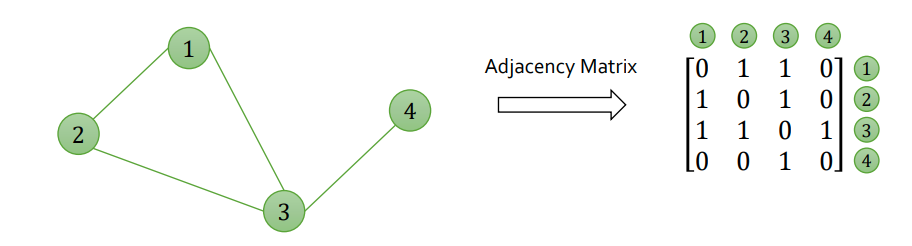
\includegraphics[width=8cm]{images/Theory-DL/AdjMat.png}
    \caption{Adjacency Matrix}
    \label{fig:AdjMat}
\end{figure}
  \item \textbf{Node Attributes or Feature Vectors (\(X\))}: Node attributes or feature vectors represent additional information associated with each node in the graph. These features can encode characteristics such as node content, properties, or embeddings. Let \( X \) denote the node feature matrix, where each row corresponds to a node and each column represents a feature dimension. For a graph with \( N \) nodes and \( D \) features, the node feature matrix \( X \) can be defined as:
  \[
  X = \begin{bmatrix} x_1^T \\ x_2^T \\ \vdots \\ x_N^T \end{bmatrix}
  \]
  where \( x_i \) represents the feature vector associated with node \( v_i \) and \( x_i^T \) denotes its transpose.
  \item \textbf{Edge Weights or Edge Attributes (\(W\))}: Edge weights quantify the strength or intensity of relationships between nodes connected by edges. These weights can represent similarity measures, distances, or any other relevant information associated with edge connections. Similar to node weights, edge weights can be learned or predefined. 
\end{enumerate}
GNNs leverage these components to perform message passing and aggregation operations across the graph structure, enabling them to capture complex relational information and make predictions based on the graph topology and node features. By integrating information from neighboring nodes and edges, GNNs can effectively model and analyze graph-structured data across various domains.
1. \textbf{Message Passing:}

Message passing is a fundamental operation in GNNs where nodes exchange information with their neighbors in the graph. This mechanism enables nodes to aggregate and propagate information across the graph, allowing them to update their representations based on the local neighborhood structure. The message passing process typically involves two main steps:

a. \textbf{Message Computation:} Each node aggregates information from its neighboring nodes to compute a message. This aggregation process involves applying a function to combine features of neighboring nodes.

b. \textbf{Message Aggregation:} After computing messages, each node aggregates the received messages to update its own representation. This aggregation operation typically involves summing or averaging the incoming messages. 

Mathematically, the message passing process can be represented as follows:
\[
m_{v \rightarrow u}^{(l)} = M^{(l)}(h_v^{(l)}, h_u^{(l-1)}, e_{vu})
\]

where:
\begin{itemize}
    \item $m_{v \rightarrow u}^{(l)}$ represents the message sent from node $v$ to node $u$ at layer $l$,
    \item $M^{(l)}$ is a message function applied to the features of nodes $v$ and $u$ and the corresponding edge $e_{vu}$,
    \item $h_v^{(l)}$ and $h_u^{(l-1)}$ are the feature vectors of nodes $v$ and $u$ at layers $l$ and $l-1$, respectively.
\end{itemize}

After computing messages, the aggregated message for node $u$ is obtained by combining messages from all neighboring nodes:
\[
m_u^{(l)} = \sum_{v \in \mathcal{N}(u)} m_{v \rightarrow u}^{(l)}
\]
where $\mathcal{N}(u)$ denotes the set of neighboring nodes of $u$.

2. \textbf{Graph Convolutions:}
Graph Convolutional Networks (GCNs) are NNs operating on graph-structured data. They extend the concept of convolutional operations from regular grid-like data, such as images, to irregular and non-Euclidean graph structures, using the graph convolution operation. The graph convolution operation involves aggregating information from neighboring nodes and updating the representations of each node based on this aggregated information. The computation of node representations in a graph convolutional layer can be expressed as follows:
\begin{equation}
h_i^{(l+1)} = \sigma\left( \sum_{j \in \mathcal{N}(i)} \frac{1}{c_{ij}} W^{(l)} h_j^{(l)} \right)
\end{equation}
where:
\begin{itemize}
\item $h_i^{(l)}$ and $h_j^{(l)}$ represent the node features (or representations) of nodes $i$ and $j$ at layer $l$, respectively.
\item $\mathcal{N}(i)$ denotes the set of neighboring nodes of node $i$.
\item $W^{(l)}$ is the learnable weight matrix for layer $l$.
\item $c_{ij}$ is a normalization factor, typically the sum of the degrees of nodes $i$ and $j$ to ensure stability and convergence.
\item $\sigma$ denotes the activation function, such as ReLU or sigmoid.
\end{itemize}
Some important aspects of Graph Convolutions are detailed below. 
\begin{enumerate}

\item \textbf{Aggregation of Neighbor Information}
The key aspect of graph convolution is the aggregation of information from neighboring nodes. Each node aggregates the features of its neighbors, weighted by the parameters learned in the weight matrix $W^{(l)}$. This aggregation process enables nodes to incorporate information from their local neighborhoods, capturing relational dependencies and structural patterns in the graph. The normalization factor $c_{ij}$ ensures that the aggregated features are appropriately scaled based on the connectivity of nodes.

\item \textbf{Weight Sharing and Parameter Efficiency}
Similar to CNNs, GCNs leverage weight sharing to ensure parameter efficiency and generalization across different regions of the graph. The weight matrix $W^{(l)}$ is shared across all nodes, allowing the model to capture common patterns and relationships present in the graph. By sharing parameters, GCNs can effectively learn representations from limited labeled data, facilitating transfer learning and adaptation to new graphs or domains.

\item \textbf{Expressive Power and Hierarchical Feature Learning}
Graph convolutional layers enable hierarchical feature learning by iteratively aggregating information from neighboring nodes. As information propagates through multiple layers, nodes can capture increasingly abstract and high-level features of the graph. The expressive power of GCNs lies in their ability to capture complex relational information and structural properties of the graph, making them suitable for various tasks such as node classification, link prediction, and graph classification.

\end{enumerate}
3. \textbf{Graph Pooling:}
Graph pooling aggregates node representations across the entire graph to compute global graph-level features and to create a coarser graph representation.
It reduces the size of the graph representation while preserving important structural and relational information. By selecting representative nodes or aggregating node features, graph pooling enables GNNs to focus on relevant information while reducing computational complexity. Graph pooling also facilitates hierarchical feature learning by allowing GNNs to operate at multiple levels of granularity, enabling the model to capture both local and global patterns in the graph. The different types of graph pooling are: 

\begin{enumerate}
\item \textbf{Top-k pooling} selects the top k nodes based on certain criteria, such as node importance or feature values, and aggregates their information to create a coarser graph representation. This method retains the most informative nodes while reducing the size of the graph, making it suitable for tasks requiring node selection or summarization.
\item \textbf{Max pooling} selects the node with the maximum feature value from each neighborhood and aggregates their information to create a coarser representation of the graph. It emphasizes the most salient nodes in each neighborhood, capturing important features while reducing redundancy.
\item \textbf{Self-attention graph pooling} leverages attention mechanisms to dynamically weight the contributions of neighboring nodes based on their importance and similarity. It allows nodes to attend to relevant information in their neighborhoods, facilitating adaptive aggregation and effective summarization of the graph. This method is particularly useful for capturing long-range dependencies and global patterns in the graph.
\end{enumerate}
Graph pooling aggregates node features to produce a compact representation of the entire graph, which can be fed into subsequent layers or used for downstream tasks. \\
Graph unpooling is a complementary operation to graph pooling, aimed at upsampling or reconstructing the original graph representation after downsampling. While graph pooling aggregates information from multiple nodes to create a coarser representation, graph unpooling aims to recover the finer details and restore the original graph structure. Some common types of graph unpooling include:
\begin{enumerate}
\item \textbf{Max unpooling} is anunpooling strategy used in conjunction with max pooling. During max pooling, the locations of the maximum activations are stored. In max unpooling, these locations serve as masks to place the pooled values back into their original positions in the unpooled feature map.
\item \textbf{Bed of nails unpooling} involves replicating or duplicating nodes from the coarse representation to reconstruct the original graph structure. In this method, unpooled nodes are placed in specific predetermined positions, often corresponding to the locations of nodes in the coarse representation. Bed of nails unpooling ensures precise restoration of the original connectivity pattern while preserving local structure.
\item \textbf{Nearest neighbor unpooling} aims to recover the original graph topology by identifying the nearest neighbors of pooled nodes in the coarse representation and reinstating unpooled nodes based on their proximity. It reconstructs edges between unpooled nodes and their nearest neighbors, restoring connectivity and preserving local structure. Nearest neighbor unpooling is effective in capturing local relationships and structural patterns in the graph.
\end{enumerate}
% \subsection{Message Passing}
% \subsection{Graph Convolutions}
% \subsection{Graph Pooling and Unpooling}
\subsection{Hierarchical Multi Resolution Approach}
Multi-grid or multi-resolution approaches in the context of GNNs involve operating on graphs at multiple levels of granularity, similar to the multigrid method in numerical analysis. 
% In extending the multi-grid concept to the GNNs, a different approach is necessary compared to Convolutional Neural Networks (CNNs). 
Unlike CNNs, where down-sampling (pooling) operators automatically coarsen the mesh, in GNNs, we create a hierarchy of meshes with increasing complexity over the domain of interest. However, traditional pooling operators used in CNNs may not be suitable for GNNs, as they focus on selecting nodes to construct a coarse graph, which is unnecessary for mesh data. Instead, we can easily define operators that transform features from one mesh to the next, either up or downward, by generating a set of meshes with varying coarsenesses.\\
Creating a mesh hierarchy involves designing meshes to subdivide the problem domain, drawing from well-established techniques in numerical analysis. One commonly used algorithm for mesh construction is Delaunay triangulation, which maximizes the minimum angle of all triangles to avoid sliver triangles. This algorithm gradually inserts new nodes into the triangulation and connects them with their neighbors under specific rules. Delaunay triangulation ensures uniform division of the domain, avoids narrow triangles, and preserves geometric properties with limited nodes. Incremental decimation is another mesh coarsening method which aims to reduce the number of points while preserving specific properties of the original mesh. It iteratively removes one vertex or edge with minimal changes until certain criteria are met. These techniques offer flexibility in creating mesh hierarchies without relying on traditional graph pooling operators, making them suitable for GNNs applied to mesh data.\\
\subsubsection{Sampling Operator}
We introduce a sampling operator for converting data between two meshes, denoted as \(M_1\) and \(M_2\), inspired by the k-nearest interpolation proposed in PointNet++ (Qi et al., 2017). Let \(z\) be a node from \(M_1\), and assume its \(k\) nearest neighbors on \(M_2\) are denoted as \(x_1, \ldots, x_k\). Let \(f\) represent some node feature. The interpolated feature \(f(z)\) is defined based on the features of \(x_i\) as follows:
\begin{equation}
  \mathbf{f}(\mathbf{z})=\frac{\sum_{i=1}^k w\left(x_i\right) \mathbf{f}\left(x_i\right)}{\sum_{i=1}^k w\left(x_i\right)} \text {, where } w\left(x_i\right)=\frac{1}{\left\|z-x_i\right\|_2}
  \end{equation}
With these operators, both up- and down-sampling operators can be defined straightforwardly for developing multi-resolution architectures for mesh based problems.
